\documentclass[11pt,dvipdfmx]{article}
%\usepackage[utf8]{inputenc}
\usepackage{deauthor,times,graphicx,url}
\usepackage{wrapfig}
%\usepackage[normalem]{ulem}
\usepackage{hyperref}
\usepackage{xcolor}
\usepackage{xspace}
%\usepackage[font=small,it]{caption}
\renewcommand\ttdefault{cmvtt}

%\graphicspath{{parameswaran/}}

\newcommand{\topic}[1]{\vspace{-3.5pt}\smallskip \smallskip \noindent{\bf #1.}}
\newcommand{\stitle}[1]{\vspace{0.5em}\noindent\textbf{#1}}
\newcommand{\emtitle}[1]{\vspace{0.3em}\noindent{\em #1}}

\newcommand{\system}{{\sf MILE}\xspace}
\newcommand{\systemLang}{{\sf MILEAGE}\xspace}
\newcommand{\helix}{{\sc Helix}\xspace}


\title{A Human-in-the-loop Perspective on AutoML:\\ Milestones and the Road Ahead}

\author{{\small Doris Jung-Lin Lee$^{\dagger*}$, Stephen Macke$^{\ddagger*}$, Doris Xin$^{\dagger*}$, Angela Lee$^{\ddagger}$, Silu Huang$^{\ddagger}$, Aditya Parameswaran$^{\dagger}$}\\
{\small \texttt{\{dorislee,dorx,adityagp\}@berkeley.edu $|$ 
\{smacke,alee107,shuang86\}@illinois.edu}}\\
{\small $^{\dagger}$University of California, Berkeley $|$  $^{\ddagger}$University of Illinois, Urbana-Champaign} $|$
{\small $^*$Equal Contribution}}

\date{June 2019}

\begin{document}

\maketitle
\vspace{-30pt}
\section{Introduction}
\par Machine learning (ML) has gained widespread adoption in a variety of real-world problem domains, ranging from business, to healthcare, to agriculture. However, the development of effective ML solutions requires highly-specialized experts well-versed in both statistics and programming. This high barrier-of-entry stems from the current process of crafting a customized ML solution, which often involves numerous manual iterative changes to the ML workflow, guided by knowledge or intuition of how those changes impact eventual performance. This cumbersome process is a major pain point for machine learning practitioners~\cite{Amershi2019,yang2018grounding} and has motivated our prior work on Helix, a declarative ML framework~\cite{xin2018helix} targeted at supporting efficient iteration. 
\par To make ML more accessible and effortless, there has been recent interest in AutoML systems, both in industry~\cite{H2O,azureAutoML,googleAutoML} and in academia~\cite{Feurer2015,olson_tpot_2018}, that automatically search over a predefined space of ML models for some high-level goal, such as prediction of a target variable. For certain tasks, these systems have been shown to generate models with comparable or better performance than those generated by human ML experts in the same time~\cite{kaggledays2019,automl}.
However, our preliminary study of ML workflows on OpenML~\cite{OpenML2013} (an online platform for experimenting with and sharing ML workflows and results) shows that AutoML is not widely adopted in practice---accounting for fewer than 2\% of all users and workflows. While this may be due to a lack of awareness  of these tools, we believe that this sparse usage stems from a more fundamental issue: {\em a lack of usability}. 
\par Our main observation is that the fully-automated setting that current AutoML systems operate on may not be a one-size-fits-all solution for many users and problem domains. Recent work echoes our sentiment that AutoML's complete automation over model choices may be inadequate in certain problem contexts~\cite{Gil2019,Wang2019}. The lack of human control and interpretability is particularly problematic when the user's domain knowledge may influence the choice of workflow~\cite{Gil2019}, in high-stakes decision-making scenarios where trust and transparency are essential~\cite{Wang2019}, and in exploratory situations where the problem is not well-defined~\cite{Cashman2018}. This trade-off between control and automation has been a century-long debate in HCI~\cite{Horvitz1999,Heer2019,Shneiderman1997,Amershi2019AI}, with modern reincarnations arising in conversational agents, interactive visual analytics, and autonomous driving. A common interaction paradigm to reconcile these two approaches is a {\em mixed-initiative} approach, where ``intelligent services and users...collaborate efficiently to achieve the user's goals''~\cite{Horvitz1999}.
\par Along the footsteps of these seminal papers, here, we outline our vision for a Mixed-Initiative machine Learning Environment (\system), by rethinking the role that automation and human supervision play across the ML development lifecycle. \system enables a better user experience, and benefits from system optimizations that both leverage human input and are tailored to the fact that \system interacts with a human in the loop. For example, our earlier work \helix~\cite{xin2018helix} leveraged the fact that workflow development happens iteratively, to intelligently materialize and reuse intermediate data products to speed up subsequent iterations. Similarly, as discussed later in this paper, leveraging user domain knowledge has the potential to drastically narrow down the exhaustive search space typically employed by existing AutoML systems. 

\begin{wrapfigure}{r}{0.6\linewidth}
    \centering
    \vspace{-10pt}    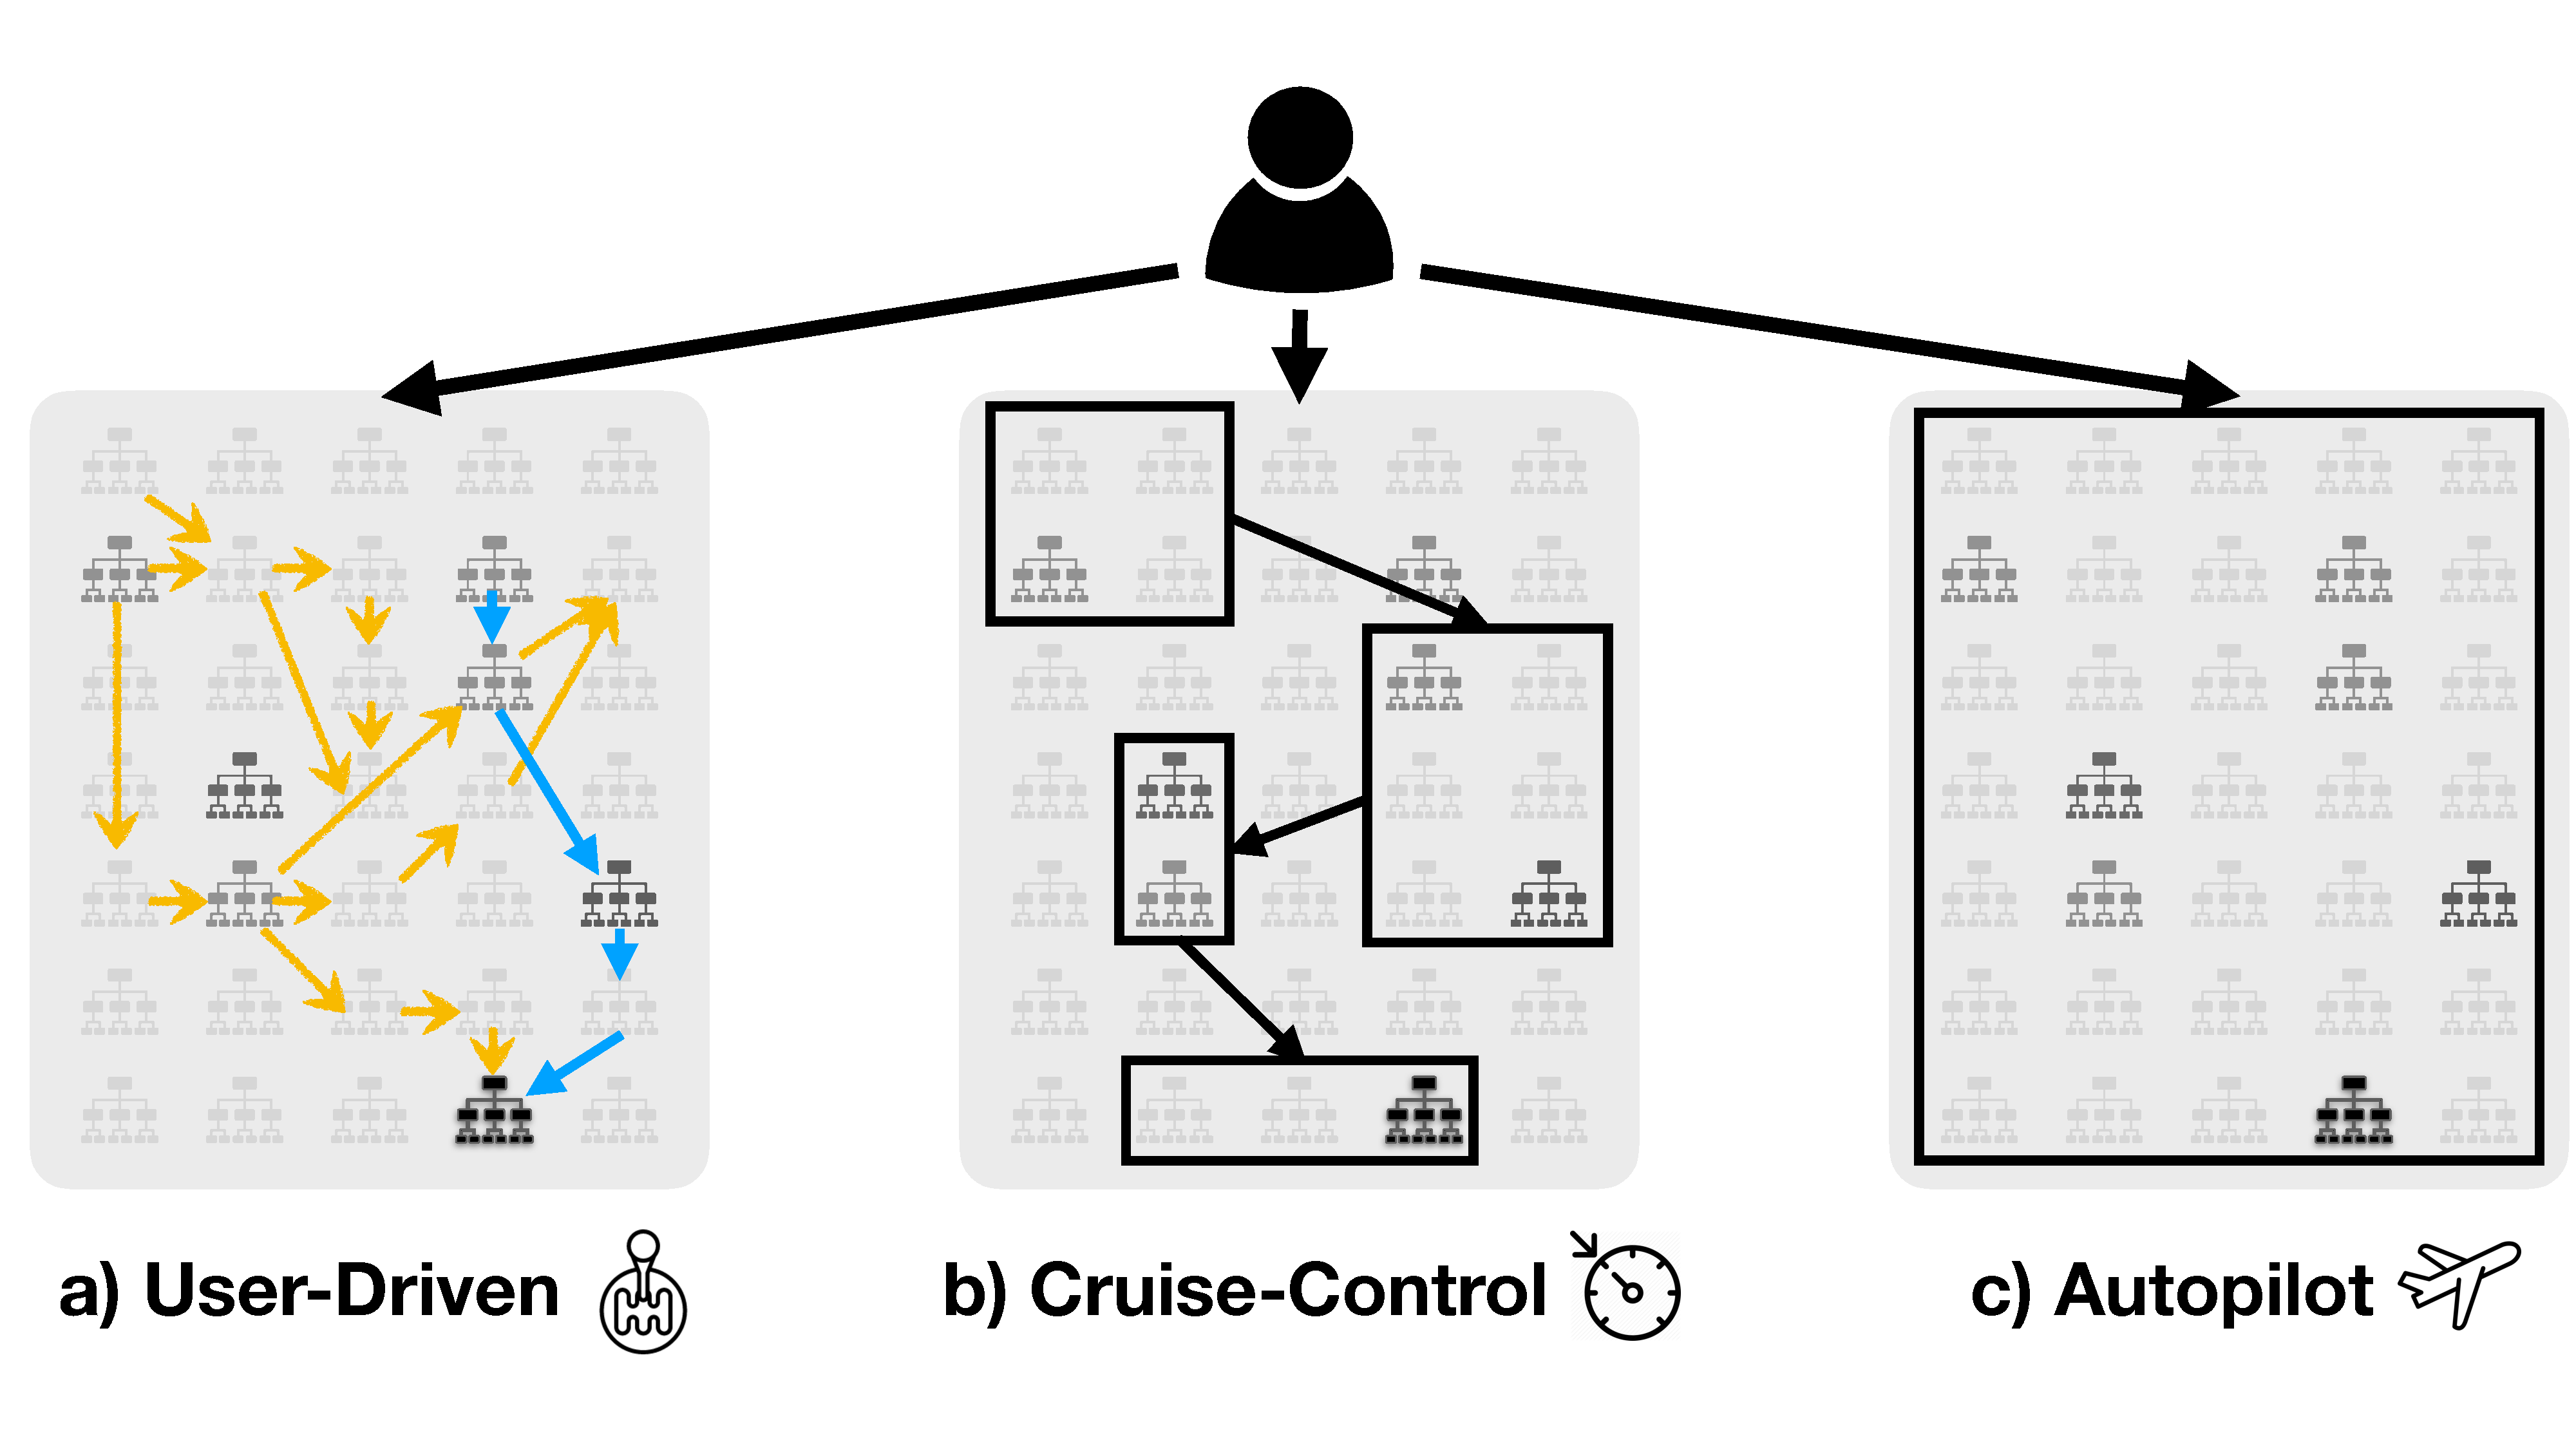
\includegraphics[width=\linewidth]{figs/ml-ieee-bulletin-fig.pdf}
    \vspace{-25pt}
    \caption{Three levels of autonomy in the ML lifecycle.
    The gray box represents the space of all possible workflows for a given task. 
    Darker workflows have better performance, and the darkest workflow at the bottom is the desired workflow.
    a) User-driven: the user has to specify the next workflow to explore in every iteration;
    a novice user (yellow arrows) might take more iterations than an expert (blue arrows)
    to reach a ``good'' workflow.
    b) Cruise-control: the user steers the system towards a set of changes (a black box) 
    to be explored automatically by the system.
    c) Autopilot: the user specifies only the dataset and the ML objective for the machine to automatically find the optimal workflow.
    }
    \label{fig:autonomy}
\vspace{-10pt}
\end{wrapfigure}

By considering the trade-offs between system acceleration and user control, we
organize our paper based on three increasing levels of autonomy---user-driven, cruise-control, and autopilot---drawing an analogy with driving. The different levels of autonomy
characterize the degree of user control and specification of problem
requirements versus the amount of system automation in identifying desired workflows (as
illustrated in Figure~\ref{fig:autonomy}). Starting from the manual, user-driven
setting (\S\ref{sec:manual}), we describe system challenges in enabling users
to rapidly try out different workflow variants, including
techniques that speed up execution time to achieve interactive responses, and
those that improve debugging and understanding of different workflow
versions. Next, in the cruise-control setting (\S\ref{sec:Mixed}), the
system works alongside users collaboratively in search of a workflow that
fits the user's needs, by letting users declaratively specifying problem requirements, and identifying desired workflows via a dialog with the user. Finally, in
the fully-autonomous, autopilot setting (\S\ref{sec:Auto}), we outline several techniques
that would improve and accelerate the search through different ML design
decisions. At a high level, these techniques hinge on {\em accelerated search}
via AutoML-aware work-sharing optimizations and {\em more intelligent search}
via knowledge captured from user-driven ML workflows.
Therefore, a holistic system for varying levels of autonomy is crucial. 
\par Our goal for characterizing the design space of such systems into the three representative levels is to bridge the knowledge gap between novice and expert users and thereby democratize the process of ML development to a wider range of end-users. For example, to build an image classifier, an expert user might want to explicitly choose which model and preprocessing techniques to use, but leaving the manual search of the hyperparameter settings to the system, whereas a novice might opt for the fully-autonomous setting to search for any optimal workflow. By addressing the research challenges in each level of autonomy, we can envision an intelligent, adaptive, multi-tiered system that dynamically adjusts to the appropriate balance between usability and customizability depending on the amount of information present in the user input. In addition, by supporting different levels of autonomy in a single system, the system can synthesize knowledge from expert users (such as knowing that a convolutional neural network would be most suitable for building an image classifier) to help the non-experts.
\par Across the different levels of autonomy, we encounter research challenges from the fields of ML, databases (DB), and HCI. The ML challenges include meta-learning techniques for intelligently traversing the search space of models. The database challenges include optimization of time and resources required for this search process leveraging common DB optimizations such as pipelining, materialization, and reuse. The HCI challenges include designing abstractions that make it easy to communicate high-level problem requirements to the system, as well as providing interpretable system outputs and suggestions. The challenges from these three fields are not isolated but instead impact each other. For example, developing DB optimizations that speed up execution time also leads to a more responsive and interactive user experience. Creating more usable debugging tools also improves model transparency and interpretability. For these reasons, in order to design a holistic solution, it is crucial to work at the intersection of these fields to tackle the challenges across the different levels of autonomy.


\begin{wrapfigure}{r}{0.6\textwidth}
\vspace{-10pt}
    \centering
    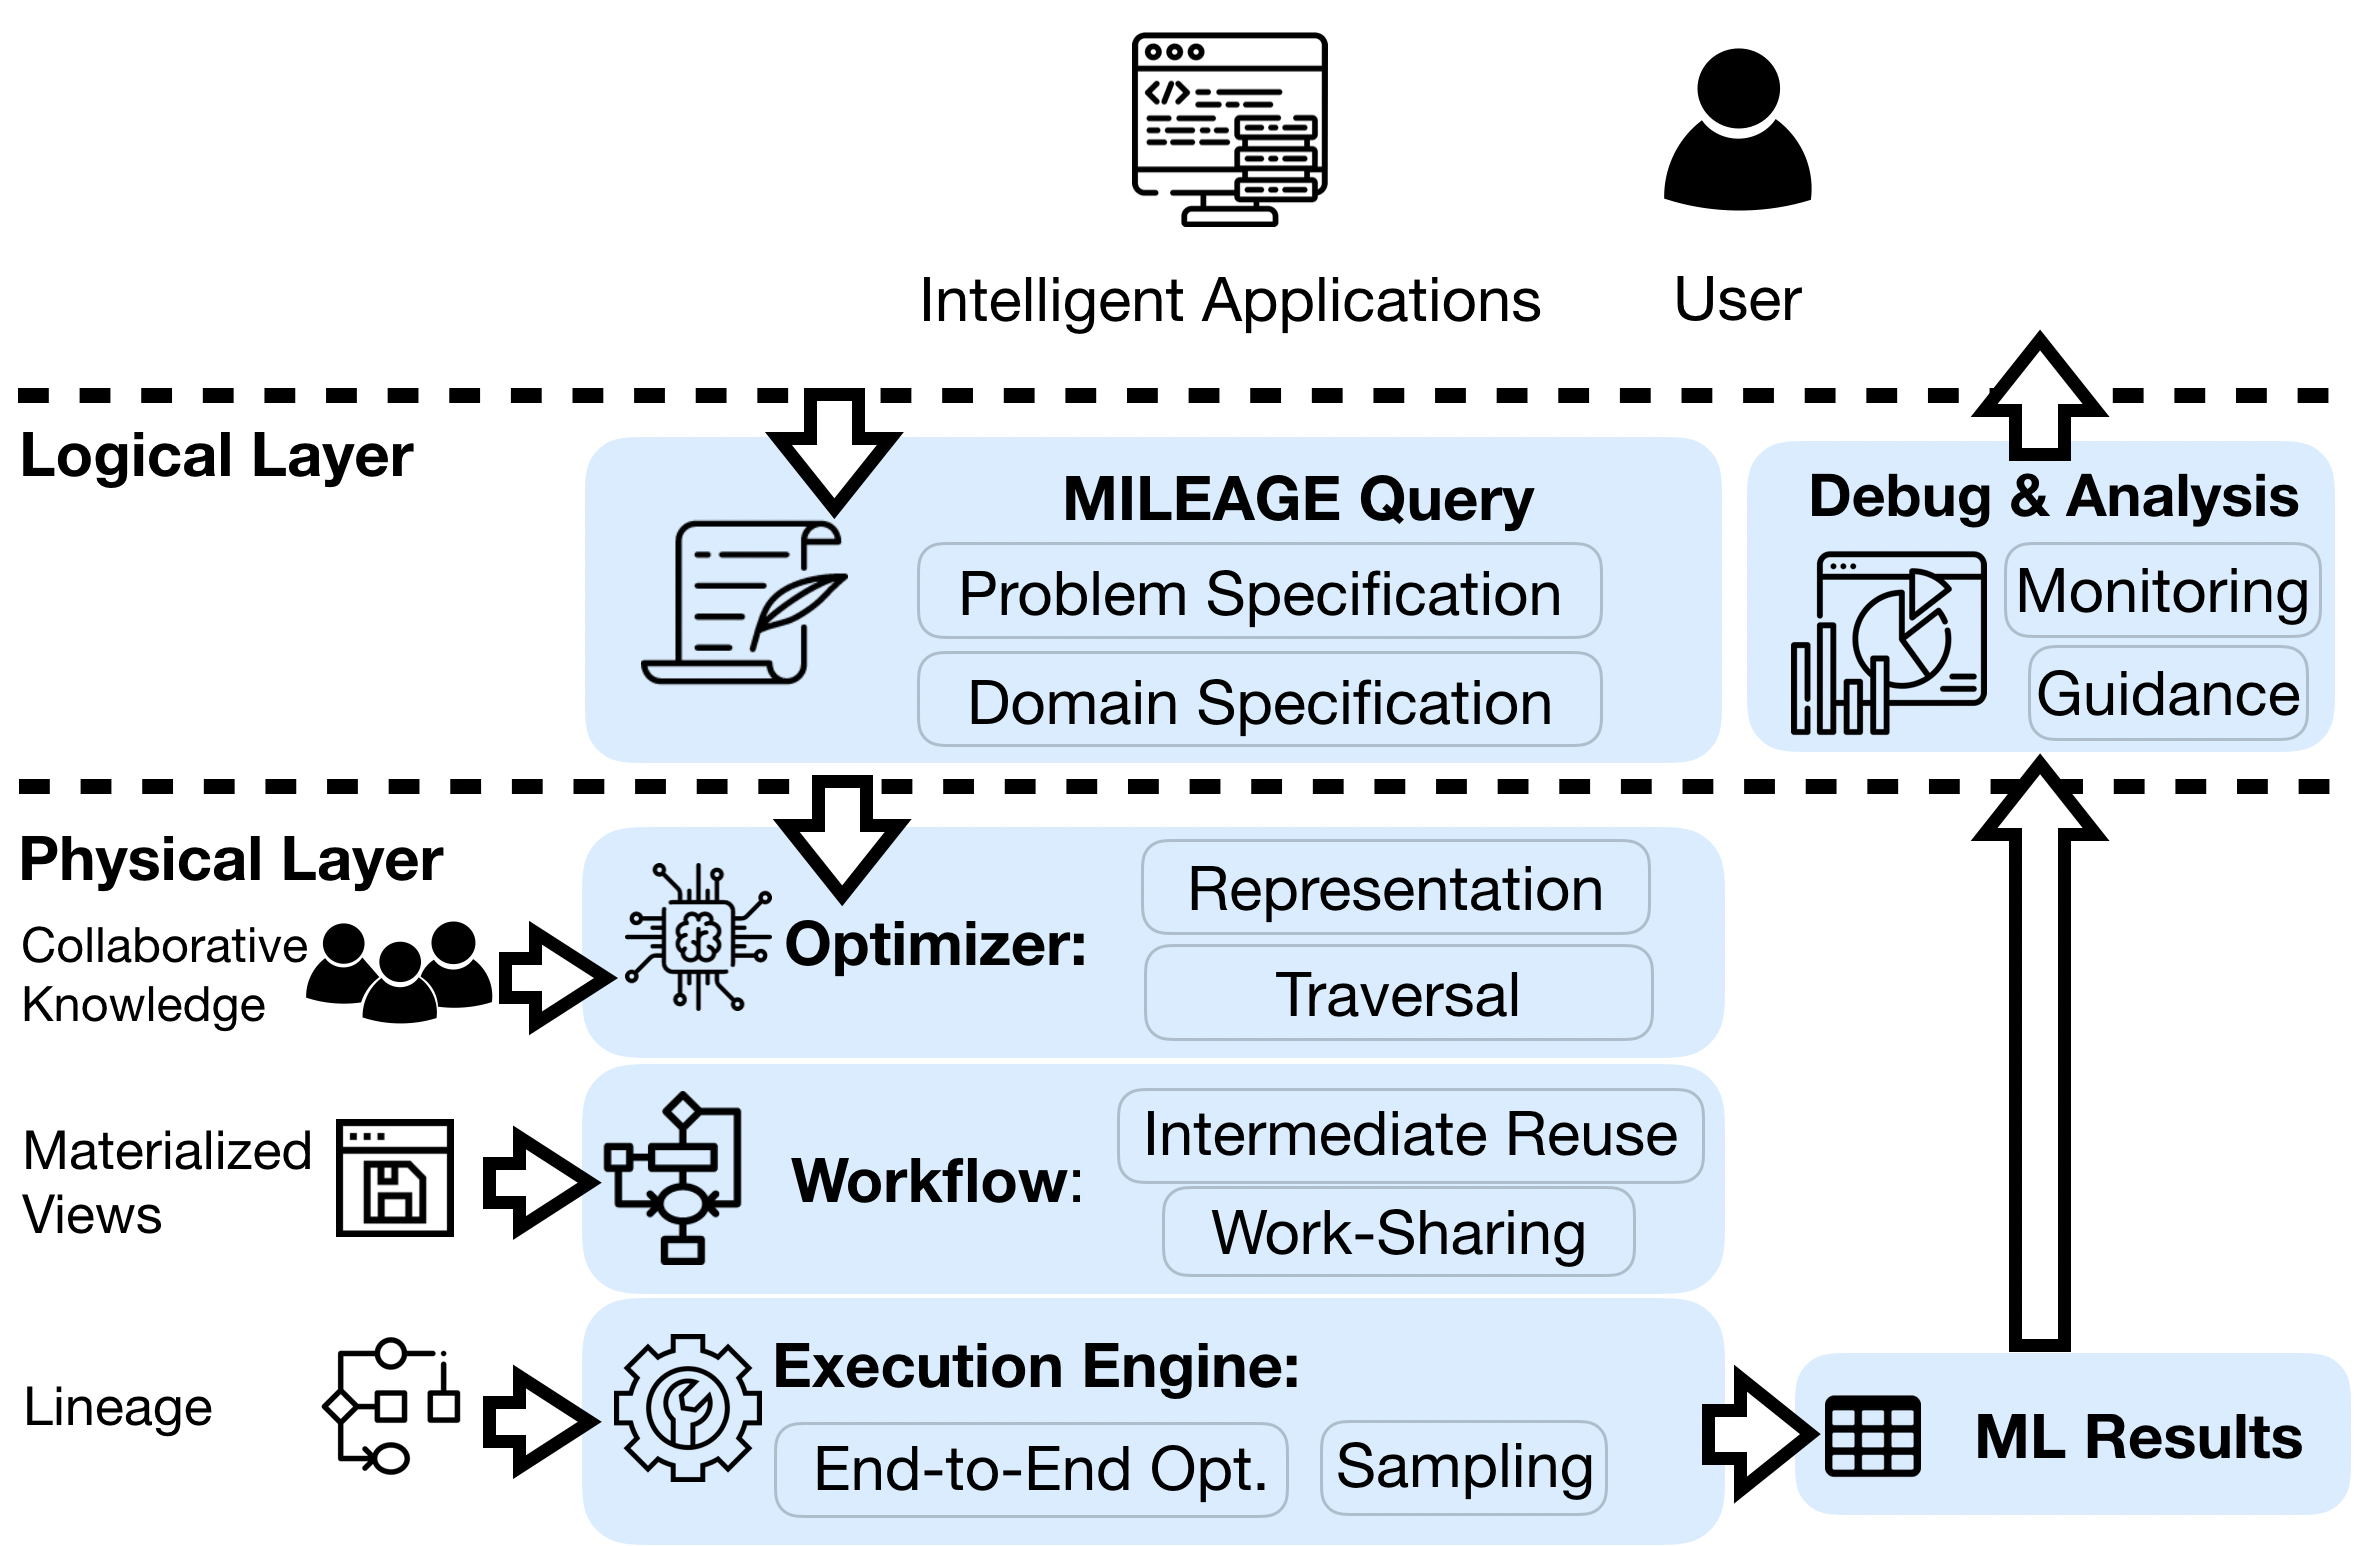
\includegraphics[width=\linewidth]{figs/architecture.png}
    \vspace{-20pt}
    \caption{\system System Overview}
    \label{fig:architecture}
    \vspace{-15pt}
\end{wrapfigure}

In our envisioned Mixed-Initiative machine Learning Environment (\system), users work collaboratively with machines in search for an optimal workflow that accomplishes the specified problem goals. As illustrated in Figure~\ref{fig:architecture}, \system is reminiscent of a relational database management system (DBMS). At the top, different application units and users can communicate with the system via a declarative ML intent query language called \systemLang (described in \S\ref{sec:Mixed}). Users do not have to use this query language directly; instead, we envision interactive interfaces that can generate such queries automatically based on user interactions (analogous to form-based interfaces generating SQL), as in our Helix IDE~\cite{helixDEMO} or TensorBoard~\cite{manetensorboard}. Given a \systemLang query, the optimizer represents and traverses through the search space defined by the \systemLang query. The output of the optimizer is a workflow, akin to a query execution plan, where the workflow's overall performance is modeled as a cost function. Similar to how operators can be reordered and pushed down to achieve the same result while optimizing for performance in an DBMS, there may be certain ML workflow choices that have equivalent results, but leads to better performance.
The obtained workflow is provided to an execution engine that performs the actions specified by the workflow, leading to a set of ML results (which can be labels for classification or a table of prediction values). Finally, the ML results are communicated back to the users for debugging and analysis.


\section{User-Driven}
\label{sec:manual}
In this setting, the user makes all the modeling decisions, 
including the initial workflow 
and iterative changes to the workflow to evaluate in subsequent iterations.
The role of the system is to help users rapidly explore the specified changes
and to track the results across iterations. 
This setting affords the users full control of the modeling process, which may be desirable for several reasons.
For example, the application has stringent security, privacy, or regulatory requirements;
or the dataset is extremely large, limiting the number of experiments that can be run.
However, since \system provides no input on modeling decisions,
this setting is more suited for expert ML users 
who demand full control of the modeling process. 
Even though expert ML users dictate the modeling iterations, 
there are many challenges associated with
focusing their attention on modeling and maximizing their productivity.
Below, we discuss concrete challenges in accelerating execution to increase interactivity 
and in helping users interpret and debug ML outputs.

\subsection{Interactivity\label{sec:interact}}
In each iteration, users rely on the results from the current and past models to make decisions about what to try next, such as a new set of features, a different model hyperparameter value, or a new model type. Shortening the execution time to obtain the model metrics and predictions would greatly improve interactivity and can be accomplished through several different system optimizations.

\topic{Materialization and reuse}
From our preliminary study of ML workflows from OpenML, 
we observed that from one iteration to the next, 
users tend to reuse a large portion of the workflow. 
About 80\% of the iterations on OpenML reuse over half of the operators from the previous iteration. 
Incremental changes, while desirable for controlled experiments with quantifiable impact, 
result in a great deal of redundant computation that can be materialized and reused in subsequent iterations to speed up iterative execution.


While materialization and reuse techniques in databases are well-studied,
applying them to ML workflows presents new challenges. 
First, na{\"i}ve solutions such as materializing all operator results can be wasteful and detrimental to performance, and reuse is not always the optimal policy. 
In some cases, recomputing from inputs can be more efficient than loading previous results.
Interdependency of materialization and reuse decisions in a workflow DAG complicates the storage and runtime tradeoff. 
For example, materializing all of the descendants of an operator $O$ precludes the need for materializing $O$, 
but $O$ needs to be loaded in a subsequent iteration if any of the descendants are modified.
Additionally, users can make arbitrary changes in each iteration. 
Making effective materialization decisions hinges upon the ability to anticipate iterative changes.

\helix investigates some of these challenges and provides heuristics for solving the problem. 
The materialization problem is proven to be NP-hard~\cite{xin2018helix}. 
As a next step, building a predictive model of what users may do next 
may help prioritize what to materialize,
given enough training data on how developers iterate on ML workflows.
OpenML is a great source for gathering such training data, 
as it records complete workflow traces.
However, a solution based purely on historical data may not respond adequately to the idiosyncrasies of a specific user---the system 
must also be able to adapt quickly to the behaviors of a new user. 
To this end, reinforcement learning (RL) can be used to explore complex materialization strategies, as others have done for query optimization~\cite{krishnan2018learning} and view maintenance~\cite{liang2019opportunistic}.


\topic{End-to-end optimization}
While materialization and reuse optimize across iterations, 
end-to-end optimization focuses on the entire workflow in a single iteration.
An important area that merits more research efforts is the joint optimization of the data-preprocessing component, (primarily relational operators) and the ML component (primarily linear algebra--or LA--operators) of the workflow. 
Relational operators deal in columns and rows, while LA operators deal in vectors and matrices. 
Although there is an intuitive correspondence between the columns and rows of a table and the columns and rows of a matrix, 
systems aimed at integrating ML into databases usually do so via a
special vector data type for performance reasons (see~\cite{kumar2017data} for a survey).
Chen et. al. propose a formal framework to unify LA and relational operators in the context of factorized ML, in which ML operators are decomposed and pushed through joins~\cite{chen2017towards}. 
Their framework can be extended to support a wider range of cross-relational and LA optimizations. 
For example, Sommer et. al. observe that sparsity arises from many sources in ML and can be exploited to optimize the execution plan for LA operators~\cite{sommer2019mnc}. 
If we were able to connect each vector position to the corresponding columns between LA and relational operators, 
we can leverage sparsity to optimize the relational portion of the workflow as well, 
e.g., automatically dropping, at the earliest opportunity, columns that correspond to zero-weight features in the ML model.
Extending the framework in Chen~\cite{chen2017towards} to support the sparsity optimization 
requires tracking additional column-wise provenance.



An orthogonal direction is to use approximation computing techniques 
such as sampling and quantization to speed up end-to-end execution 
for rapid feedback to users regarding the quality of the current workflow. 
For sampling, one needs to ensure that the sample is representative of the underlying dataset 
and that the same sample is used throughout the workflow, ideally without modifying existing operators.
Quantization pertains to using imprecise weights represented by fewer bits to obtain model performance comparable with the full-precision version~\cite{hubara2017quantized}.



\subsection{Interpretability and Debuggability}
Another important aspect of helping users make modeling decisions is 
assisting in the analysis of the \textit{artifacts} involved in the modeling process, 
including input data, intermediate results of operators within the workflow, models, and outputs~\cite{Garcia2018}.
Deciding on effective iterative changes requires a thorough understanding of the behavior of the current model. 
To make sense of existing models, 
users might need to examine a number of artifacts and the relationships between them. 
For example, to debug a bad prediction, the user might look at the model and
the most relevant training examples
that led to the prediction.
This process requires tracking a combination of coarse-grained and fine-grained lineage across related artifacts.

\topic{Coarse-grained}
Artifacts in this category include workflow versions and the metadata associated with each version, such as model hyperparameters and performance metrics. 
A number of systems 
have been developed to facilitate the recording of iterative workflow versions and metadata~\cite{vartak2016m,zaharia2018accelerating,Garcia2018}. 
These systems enable tracking via user-specified logging statements injected into their workflow programs.
The goal is to be minimally intrusive and lightweight---the system does not need to provide special implementations for each existing operator since the user specifies the metrics of interest explicitly. 
However, a more automatic solution to log metadata can leverage a combination of data lineage tracking and program analysis. 
Schelter et. al. propose a declarative language for users to specify logging at the operator and workflow level instead of by individual metrics~\cite{schelter2017automatically}.
We envision taking this one step further and completely automating the tracking of metadata, by injecting logging statements inside the compiler via program analysis.
With the ever-growing body of ML frameworks, it is not scalable to implement solutions specific to each framework. 
Instead, we should focus on common model representations, such as PMML\footnote{\url{http://dmg.org/pmml/v4-3/GeneralStructure.html}} and ONNX\footnote{\url{https://onnx.ai/}}, that are easily portable across frameworks,
akin to how LLVM handles many different languages with a unified intermediate representation (IR) for analysis. 
The model IRs have unified representations of operator parameters and input/output types, as well as mechanisms for users to annotate operators, which can be leveraged to specify custom logging requirements. 


\topic{Fine-grained}
As mentioned previously, fine-grained data lineage is helpful for diagnosing model issues,
e.g., tracing back to the input data that led to a particular bad prediction.
Supporting fine-grained data lineage in data-intensive, ad-hoc analysis is challenging for several reasons:
1) the amount of possible lineage data to track is often combinatorial with respect to the raw data;
2) the workloads are unpredictable; and
3) query results need to be served in real-time. 
The common technique to address 3) is to leverage results precomputed offline,
but 2) makes it difficult to predict what precomputation would be beneficial 
and 1) makes it infeasible to precompute all possible results in the absence of predictability.
We identify three promising directions that can effectively address all three confounding challenges.


During debugging, users create a great deal of \textit{ephemeral knowledge} 
that could potentially help with future debugging but is currently wasted. 
For example, a user runs a query to find outlier values for a given column. 
The next time someone else needs to debug an application using data from the same column, 
the outliers could potentially help explain anomalous behaviors, 
or the system could recommend outliers as a diagnostic for a different column for related issues.
Aghajanyan et. al.~\cite{aghajanyan2019signal} propose a system for capturing insights from these exploratory workloads to assist with future debugging. 
Doing so not only reduces redundant computation but also makes future workloads more regular by guiding user exploration with predefined operations.
Consequently, the system can selectively store a small subset of fine-grained lineage most likely to accelerate user-interactivity during debugging in a cost-effective manner.
Research in systematizing ad-hoc workloads into knowledge that assists with future debugging is still nascent and warrants further investigation.

Even with selective storage, the amount of fine-grained lineage data is still potentially huge 
and requires carefully designed storage schemes.  
In \helix, we have begun to explore storing lineage in the materialization of workflow intermediates. 
The idea is that while it is prohibitive to store the fine-grained input-output relationship 
for every single operator in the workflow,
we can selectively store only the output of expensive operators 
and replay the cheap operators on top of materialized intermediates to recover the full lineage.
For serving fine-grained lineage in real-time, SMOKE~\cite{psallidas2018smoke} is 
an in-memory database for serving fine-grained lineage for relations operators
at interactive speed,
using heuristics to solve the problem of materialization and replay explored in \helix.
Whether SMOKE or the techniques within can be generalized for ML operators and to dataset that do not fit in memory posits interesting research challenges.



\section{Cruise-Control}
\label{sec:Mixed}
Unfortunately, the fully user-driven setting is the modus operandi for ML application development supported by the majority of existing tools, irrespective of user expertise. 
In this section and the next, we explore system designs to help change the landscape of ML tooling, making it more accessible to a wider range of users.

In the cruise-control setting, the user specifies their problem requirements and any domain-specific knowledge to \system. \system then automatically searches through the space of potential workflow options and recommends an acceptable workflow that meets the specification, via a dialog with the user.  Since the technology for recommending acceptable/accurate models overlaps heavily with that the model search capabilities in the autonomous setting (\S\ref{sec:Auto}), here, we focus our discussion on the challenges associated with designing the appropriate logical representation of the model space that the end-user interacts with. This logical representation abstracts away the underlying details of how the search and inference are performed, so that changes or additions of new search strategies and models would not affect end-user experience. As  in Figure~\ref{fig:architecture} and described in this section, the logical representation consists of two components to facilitate a dialog between  user and  system (akin to a dashboard). From user to system, we first describe a language that enables users to express their ML `intent'. Then, going from system to user, we discuss interfaces that communicate system outputs to the user.
\subsection{Declarative Specification of ML Intent}
Unlike traditional programming where the problem solution is deterministic, since ML is data-dependent, even an expert will only have a vague impression of what their optimal workflow would look like, based on their desired properties for the eventual model outputs. However, users often have some preferences, constraints, requirements,  and knowledge regarding the problem context (collectively referred to as \emph{intent}) constraining the space of potential model solutions. We will first describe two characteristics of ML intents (ambiguity and multi-granularity) that presents research challenges in operationalization. We illustrate these characteristics via a hypothetical example of a user developing a cancer diagnostic model based on clinical data. Next, we describe our proposed solution strategy in developing a declarative language, \systemLang, that enable users to specify their ML intent. While prior work has proposed declarative specification of ML tasks~\cite{kraska2013mlbase} and feature engineering processes as UDFs~\cite{Anderson2013}, these endeavors have been focused on a specific aspect of the ML lifecycle. We argue for a holistic view that enables users to express a wide range of high-level, nuanced ML intents to the system.

\topic{Ambiguous Intents}
Our first challenge is that ML intents can often be \emph{ambiguous}---in other words, high-level, qualitative problem requirements are ambiguous and often do not translate exactly to a low-level workflow change (e.g., hyperparameter setting, preprocessing choice). For instance, in the cancer diagnostic example, the ML developer might indicate that the desired model should be interpretable to physicians and patients alike. In addition, since records are transcribed by human clinicians, the model must be robust to noisy and potentially erroneous data inputs, as well as missing values.  Another reason why ML intents can be ambiguous is that problem requirements often stem from `fuzzy' domain-specific knowledge. For example, an oncologist may indicate that because lung cancer is more fatal (higher mortality rates) than other types of cancer, false negatives should be penalized more heavily in the lung cancer diagnosis model. There are many potential approaches to operationalize these and other similar problem requirements, including modifying regularization, developing a performance metric beyond traditional classification accuracy, or choosing a model that is robust to class imbalance. The challenge therefore lies in understanding how can we can map these ambiguous high-level problem requirements to suggest some combination of workflow changes.

\topic{Multi-Granularity Intents}
Another challenge in designing an ML intent language is that user requests are \emph{multi-granularity}, encompassing a variety of different input types at different levels of granularity. At the highest level, a user can specify problem requirements, goals, or domain knowledge; at an intermediary level, users can refine or prune out portions of the search space (ranges of parameter options), at the lowest level, users can fix specific preprocessing procedures or hyperparameter values (similar to what one would do in the user-driven setting). The multi-granularity nature of ML intent stems from users with different expertise levels. For example, a clinician might only be able to specify the desired task goal (e.g., predict attribute `mortality rate'), whereas an ML expert might have more specific model requirements (e.g., use a random forest with 10-50 trees, max tree depth of 4-8, with entropy as split criteria). The research challenge lies in developing a specification framework that can adapt and jointly perform inference based on signals from different granularities, as well as appropriate interfaces to elicit different input requirements from users. Both of these challenges demand a more holistic understanding of the interdependencies and impact of different ML design choices, and how they affect the resulting workflow characteristics.

\topic{\systemLang Improvements}
Our proposed solution is to develop \systemLang, a declarative specification language that
allows users to communicate their ML intent to the system. \systemLang needs to be able to interpret two different types of specifications,
requests regarding problem details and requests involving domain knowledge.
Existing AutoML systems often require some form of problem
specification~\cite{H2O,azureAutoML,golovin2017google}, but do not account for domain specification. Domain specification consists of domain-specific
knowledge that influences workflow decisions, such as the knowledge about
mortality rates of different types of cancer and the presence of noisy and
missing values in the data collection process. While problem specification is
a required component of the query, domain specification is optional
information that is helpful for improving the model. Together, the \systemLang query
consisting of domain and problem specification causes the system to search
through potential workflow options, with the system returning a ranked list of
optimal workflows. Each of these workflows may be conveniently specified
through something declarative like the Helix-DSL~\cite{xin2018helix}, or be
compiled into imperative scripts (such as TensorFlow and Scikit-Learn). 

Further drawing from the analogy with SQL for
DBMS, we outline several desired properties in
the language design for such a system. Starting from the top of the stack in
Figure~\ref{fig:architecture}, the declarative language should act as a logical
representation that supports physical independence with respect to how the
search is actually done under-the-hood. Since ML research and practice is
fast-paced and highly-evolving, the logical representation established by the
declarative language ensures that if we have new representations, models,
knowledge sources, or search strategies, the underlying changes can be
completely hidden away from end-users. The declarative language also serves as
a common, unifying exchange format across different end-user applications.
Apart from the logical representation of the task definition in the problem
specification, there are additional language components for specifying views
and constraints.
\emph{View definitions} specify what intermediate output from the workflow can
be materialized and reused in the later part of the workflow.
Views can be defined explicitly by the user or by an intelligent
application (such as Helix~\cite{xin2018helix}, DeepDive~\cite{Shin2015}) to
create and materialize views. The intelligent application keeps track of what
has been materialized and notifies the optimizer to reuse any views that are
already materialized whenever appropriate.
\emph{Constraints} are parts of the problem specification that limits certain
portions of the solution search space, in order to ensure the consistency and
validity of the resulting workflow. These constraints may be in the form of
performance requirements, some measure of model robustness or fairness (e.g.,
checking that training data is not biased towards a particular racial group),
or specifying the latency budget allocated to search. Both the view and
constraint specification are optional declarations as part of the language and
accounted for inside the optimizer. 
\subsection{Communicating System Suggestions to Users}
\par While the declarative query language enables users to communicate their intents to the system, there is also research challenges in the reverse direction, in communicating system suggestions to users. In this section, we briefly outline several important unsolved research problems related to how the system communicates suggestions to: 1)
guide users towards better workflow decisions (guidance) and 2) correct and prevent users from overlooking potential model errors (correction). 

\topic{Guidance Towards Optimal Workflow Decisions}
Given a declarative specification of ML intent, the system automatically
traverses through the search space and returns suggestions regarding the
workflow choices. Existing human-in-the-loop AutoML
systems~\cite{Wang2019,Cashman2018} feature visualizations for model
comparison, with users able to assign a computational budget to the
AutoML search, specify the search space and model choices, or modify the
problem specification. It remains an open research question as to what types
of workflow recommendations and end-user interaction for model-steering would
be most useful to users. What is the appropriate
granularity of feedback to provide to the user that would be useful in guiding
them towards an optimal workflow? Should we be suggesting modifications to an
existing workflow, offering users to chose between multiple workflows, or
recommending the entire workflow?
Moreover, what
aspects of the workflow development phase require the most amount of guidance
and assistance? For example, while most AutoML systems have focused on model
selection and hyperparameter search, it may possible that users actually need
more assistance with feature engineering or data preprocessing. One of our
goals in studying workflows on OpenML is to understand where existing ML
developers struggle the most in the development lifecycle (spending most
amount of time or with minimal performance gains). These observations will
guide our work to address existing pain-points in the ML development lifecycle.
A far-reaching research question is to examine whether workflow
recommendations from a well-designed guidance system have the potential to
educate novice users about best practices in model development. These best
practices can include knowledge about what model to pick over another in 
certain scenarios or preprocessing techniques when the input data
exhibits certain characteristics. The recommendation system acts as a personal
coach that could teach the user practical ML skills while they are performing
an ML task.

\topic{Corrective Suggestions via Proactive Monitoring}
Many recent examples pervasive in the media have highlighted how errors from
production ML system can have detrimental and unintended consequences, from
systematic biases in a recidivism
predictions\footnote{\url{https://www.propublica.org/article/machine-bias-risk-assessments-in-criminal-sentencing}}
to racist and vulgar responses in a public
chatbot\footnote{\url{https://en.wikipedia.org/wiki/Tay_(bot)}}. To this end,
several systems have been proposed to validate and monitor the quality of
production ML workflows
~\cite{Breck2019,Schelter2018,Chung2018}. These systems monitor
the model and raise a red-flag when the result from the deployed ML pipeline
is potentially erroneous (e.g., when the input data distribution changes
drastically).
If done properly, the proactive monitoring capabilities of
\system may the potential for enhancing user's trust in the final ML model
that is developed, improve the overall production model quality, and reduce
the cost of model maintenance.

\section{Autopilot}
\label{sec:Auto}
Depending on the user's level of expertise, they
may wish to maintain some degree of control (Figure~\ref{fig:autonomy}b), steering
\system between portions of the search space, or they
may wish to delegate the entire search process to \system (Figure~\ref{fig:autonomy}c),
letting it decide how and where to search. 
Doing this correctly would be the ``holy grail'' of AutoML:
a general, hands-free technology capable of producing
an ML workflow with adequate performance, within a given time or resource budget.

We described some of the challenges associated with exposing
these capabilities to the user in the previous section; in this section, we
focus on the system side. The major difficulty associated with driverless
AutoML is that the design space of possible ML workflows suffers from a combinatorial curse
of dimensionality. Therefore, the challenge is: {\em how do
we make the AutoML search process over this design space as efficient as possible?}

There exists an enormous breadth
of work from the AutoML community on how to best automate hyperparameter
search~\cite{bergstra2011algorithms,bergstra2012random,golovin2017google}, 
how to warm-start hyperparameter search~\cite{feurer2014using,fusi2018probabilistic,gomes2012combining},
how to learn how to select good workflow
{\em configurations}\footnote{An ML workflow configuration is comprised of the hyperparameter and other settings determining the workflow's behavior.}
\cite{brazdil2003ranking,todorovski2002ranking},
how to trade-off model performance and search time by modeling the time
budget into multicriterion optimization problems, and even how to learn the structure
of neural architectures~\cite{pham2018efficient,zoph2016neural} and other ML workflows.
We foresee that \system, which
caters to multiple levels of expertise,
can gather additional data on effective ML workflows from expert users
(beyond the traces available in public metadata repositories such as
OpenML~\cite{OpenML2013}),
or ``meta-features'', that can then be leveraged by existing meta-learning techniques.
Beyond these existing techniques for {\em smarter search}, we envision that \system will apply
ideas from the DB community for {\em faster search}.
We propose two concrete realizations of this vision:
First, \system can work in tandem with
AutoML search strategies
that operate on progressively larger samples of training data in order to evaluate the
``goodness'' of particular configurations.
In many cases, intermediates computed on smaller training data samples can be reused for larger samples.
These optimizations are inspired by prior work
for employing smart caching and reuse in large-scale~\cite{Sparks:EECS-2016-200} and
iterative~\cite{xin2018helix,Shin2015} ML workflows for future use.
Second, for AutoML,
we often know an entire up-front {\em set} of ML workflow configurations,
unlike the iterative development setting explored in Helix~\cite{xin2018helix}
where the configurations are
revealed one-by-one. As such,
\system can identify and exploit opportunities
for {\em workload sharing}, whereby multiple workflows are combined, thereby making better use of locality and data parallelism.
We describe these two directions next.

\topic{Progressive Intermediate Reuse}
\label{sec:progreuse}
Some modern, {\em multi-fidelity} Hyperparameter Optimization (HPO) techniques
approximately evaluate the generalization ability of ML workflow configurations by
training on samples of the training data; see~\cite{huang2018efficient,kohavi1995automatic,provost1999efficient}
for examples. If a configuration $C$ is promising on a subset $S$ of the training
data, it might then be evaluated on a larger subset $S'$ of training data.
How can we use the work already done for $C$ on $S$ to speed up training on $S'$?

We propose that any processing composed of {\em associative operations} can be
reused when increasing the training data size. To give a concrete example,
consider PCA, which computes principal components via a singular value decomposition
on the feature covariance matrix. To compute the principal components for the set of feature values associated with $S'$,
we first need a corresponding covariance matrix for $S'$. If we only have the covariance matrix for $S$
without any additional information, it is not enough to help us compute $S'$ --- we must start from scratch
and perform a full pass over the training data. However, if we cache counts, sums, and pairwise dot products
for features in $S$, we can update these cached quantities with {\em only the data in $S'\setminus S$},
thanks to the associativity of $(+)$, after which we can proceed with the SVD as normal.

The major research challenge is to develop an optimizer that automatically identifies
computations composed of associative operations. The output of such operations can be cached between runs
on successively larger subsets of the training data, leading to potential speedups.


\begin{wrapfigure}{l}{0.55\textwidth}
\vspace{-10pt}
    \centering
    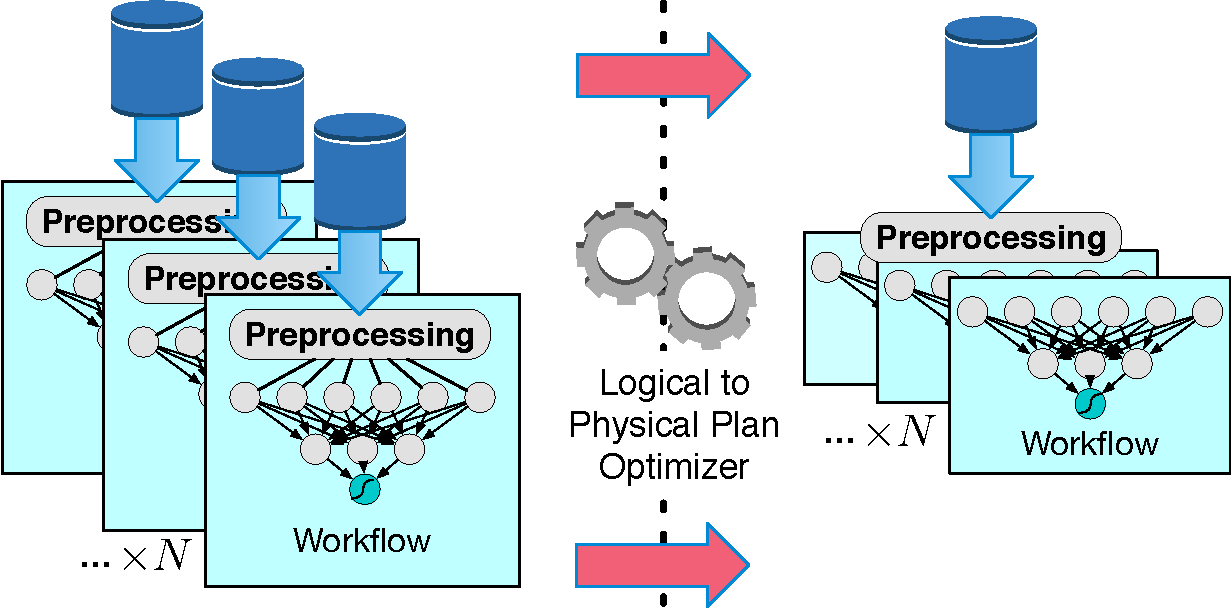
\includegraphics[width=\linewidth]{figs/workshare.pdf}
    \vspace{-15pt}
    \caption{\footnotesize Compiling a logical specification of multiple workflow configurations to a physical work-sharing plan.}
    \label{fig:workshare}
    \vspace{-10pt}
\end{wrapfigure}
\topic{Work-Sharing Optimizations}
\label{sec:sharing}
AutoML search strategies typically must select from a number of ML workflow configurations.
The space of configurations to evaluate, however, is typically high-dimensional.
Blackbox HPO methods like
grid search and random search~\cite{bergstra2012random} must perform large
numbers of workflow evaluations, and even multi-fidelity methods
like successive halving~\cite{jamieson2016non}, Hyperband~\cite{li2016hyperband}
and ABC~\cite{huang2018efficient} that leverage approximation to speed up workflow evaluation
must still try out a large number of hyperparameter configurations.

Our key observation is that, at least in some cases, the configurations share
a large amount of identical computation. This, in turn, can be exploited to
reduce I/O and memory latency by {\em using the same training batches to train
multiple models simultaneously}.
Although any single model will train more slowly than if it were to receive dedicated
hardware resources, an ML workflow in which $N$ models are trained concurrently
will be faster than separate workflows for which each model is trained in series.
Furthermore, if the training batches are preprocessed on-the-fly, the preprocessing
need only be done once for concurrent training, compared to $N$ times for serial training.

Though this technique should generalize to many kinds of ML workflows,
we envision that it will be especially fruitful
for training multiple neural network configurations simultaneously.
As GPU and TPU accelerators increase in speed, memory
capacity, and memory bandwidth, it is increasingly challenging
for CPU cores to handle ETL tasks (reading from disk, parsing,
shuffling, batching) so as to maximize accelerator utilization.
Giving these accelerators more work is one way to alleviate this bottleneck.

This observation thus motivates the research direction
of compiling a {\em logical} specification of a set of ML workflow
configuration evaluations into a {\em physical} representation optimized for
locality and data parallelism.
Our multi-configuration physical planner is illustrated abstractly in Figure~\ref{fig:workshare}.

Although the kinds of work-sharing optimizations described
have the potential to accelerate search through hyperparameter configurations, we foresee
some difficulties along the road. First of all, \system will need to facilitate work-sharing
without requiring separate, bespoke implementations of ML models specialized for work-sharing.
Secondly, we foresee that it will be
nontrivial to make these work-sharing strategies operate with existing strategies to avoid
overfitting to a fixed validation set. For example, one strategy~\cite{levesque2018bayesian} uses a separate shuffling
of the training and validation splits for each workflow configuration to avoid overfitting to
a static validation set. Employing such a strategy in concert with work-sharing optimizations will
require careful maintenance of additional provenance information during training, so that some configuration $C$
knows to selectively ignore the examples that appear in other configurations' training
splits but also appear in $C$'s validation split.


\section{Conclusion: Going the Extra \system}
\label{sec:conclusion}
Present-day ML is challenging: not everybody can get mileage out of it. 
While AutoML is a step in the right direction, there are many real-world settings
that require fine-grained human supervision.
We propose \system, an environment
where humans and machines together drive the search for desired ML solutions.
We identified three settings for \system representing
different levels of system automation over the design space of ML workflows---user-driven, cruise-control, and autopilot. 
The hope is that regardless of your desired setting, \system gets you there faster.
By catering to users with different levels of expertise, 
we hope to pool their collaborative experience in improving search heuristics. 
We also explore research opportunities in accelerating execution 
by applying traditional database techniques, such as materialization, lineage-tracking, and work-sharing. 
We hope that our \system vision serves as a roadmap for researchers to 
address the valuable opportunities that stem from humans-in-the-loop of the machine learning lifecycle.

{\small
\begin{thebibliography}{10}

\bibitem{azureAutoML}
{Automated ML algorithm selection \& tuning - Azure Machine Learning service}.
\newblock
  \url{https://docs.microsoft.com/en-us/azure/machine-learning/service/concept-automated-ml}.

\bibitem{H2O}
{AutoML: Automatic Machine Learning}.
\newblock \url{http://docs.h2o.ai/h2o/latest-stable/h2o-docs/automl.html}.

\bibitem{aghajanyan2019signal}
S.~Aghajanyan, R.~Batoukov, and J.~Zhang.
\newblock {Signal Fabric{\textemdash}An AI-assisted Platform for Knowledge
  Discovery in Dynamic System}.
\newblock Santa Clara, CA, 2019. {USENIX} Association.

\bibitem{Amershi2019}
S.~Amershi, A.~Begel, C.~Bird, R.~DeLine, H.~Gall, E.~Kamar, N.~Nagappan,
  B.~Nushi, and T.~Zimmermann.
\newblock Software engineering for machine learning: A case study.
\newblock IEEE Computer Society, May 2019.

\bibitem{Amershi2019AI}
S.~Amershi et~al.
\newblock {Guidelines for Human-AI Interaction}.
\newblock {\em CHI 2019}, pages 13--26.

\bibitem{Anderson2013}
M.~Anderson et~al.
\newblock {Brainwash: A Data System for Feature Engineering}.
\newblock {\em CIDR}, 2013.

\bibitem{bergstra2012random}
J.~Bergstra and Y.~Bengio.
\newblock Random search for hyper-parameter optimization.
\newblock {\em Journal of Machine Learning Research}, 13(Feb):281--305, 2012.

\bibitem{bergstra2011algorithms}
J.~S. Bergstra, R.~Bardenet, Y.~Bengio, and B.~K{\'e}gl.
\newblock Algorithms for hyper-parameter optimization.
\newblock In {\em Advances in neural information processing systems}, pages
  2546--2554, 2011.

\bibitem{brazdil2003ranking}
P.~B. Brazdil, C.~Soares, and J.~P. Da~Costa.
\newblock Ranking learning algorithms: Using ibl and meta-learning on accuracy
  and time results.
\newblock {\em Machine Learning}, 50(3):251--277, 2003.

\bibitem{Breck2019}
E.~Breck, N.~Polyzotis, S.~Roy, S.~E. Whang, and M.~Zinkevich.
\newblock {Data Validation For Machine Learning}.
\newblock {\em Sysml}, 2019.

\bibitem{Cashman2018}
D.~Cashman, S.~R. Humayoun, F.~Heimerl, K.~Park, S.~Das, J.~Thompson, B.~Saket,
  A.~Mosca, J.~Stasko, A.~Endert, M.~Gleicher, and R.~Chang.
\newblock {Visual Analytics for Automated Model Discovery}.
\newblock {\em arXiv:1809.10782}, 2018.

\bibitem{chen2017towards}
L.~Chen, A.~Kumar, J.~Naughton, and J.~M. Patel.
\newblock Towards linear algebra over normalized data.
\newblock {\em Proceedings of the VLDB Endowment}, 10(11):1214--1225, 2017.

\bibitem{Chung2018}
Y.~Chung, T.~Kraska, N.~Polyzotis, and S.~E. Whang.
\newblock {Slice Finder: Automated Data Slicing for Model Interpretability}.
\newblock {\em SysML}, pages 1--13, 2018.

\bibitem{feurer2014using}
M.~Feurer et~al.
\newblock Using meta-learning to initialize bayesian optimization of
  hyperparameters.
\newblock In {\em Proceedings of the 2014 International Conference on
  Meta-learning and Algorithm Selection-Volume 1201}, pages 3--10. Citeseer,
  2014.

\bibitem{Feurer2015}
M.~Feurer et~al.
\newblock {Efficient and robust automated machine learning}.
\newblock In {\em NeurIPS'15}, 2015.

\bibitem{fusi2018probabilistic}
N.~Fusi, R.~Sheth, and M.~Elibol.
\newblock Probabilistic matrix factorization for automated machine learning.
\newblock In {\em Advances in Neural Information Processing Systems}, pages
  3348--3357, 2018.

\bibitem{Garcia2018}
R.~Garcia, V.~Sreekanti, N.~Yadwadkar, D.~Crankshaw, J.~E. Gonzalez, and J.~M.
  Hellerstein.
\newblock Context: The missing piece in the machine learning lifecycle.
\newblock In {\em KDD CMI Workshop}, volume 114, 2018.

\bibitem{Gil2019}
Y.~Gil et~al.
\newblock Towards human-guided machine learning.
\newblock In {\em IUI '19}, pages 614--624, New York, NY, USA, 2019. ACM.

\bibitem{golovin2017google}
D.~Golovin et~al.
\newblock Google vizier: A service for black-box optimization.
\newblock In {\em SIGKDD'17}, pages 1487--1495. ACM, 2017.

\bibitem{gomes2012combining}
T.~A. Gomes, R.~B. Prud{\^e}ncio, C.~Soares, A.~L. Rossi, and A.~Carvalho.
\newblock Combining meta-learning and search techniques to select parameters
  for support vector machines.
\newblock {\em Neurocomputing}, 75(1):3--13, 2012.

\bibitem{googleAutoML}
Google.
\newblock {AutoML Tables}.
\newblock \url{https://cloud.google.com/automl-tables/}.

\bibitem{Heer2019}
J.~Heer.
\newblock {Agency plus automation: Designing artificial intelligence into
  interactive systems}.
\newblock {\em Proceedings of the National Academy of Sciences},
  116(6):1844--1850, 2019.

\bibitem{Horvitz1999}
E.~Horvitz.
\newblock {Principles of mixed-initiative user interfaces}.
\newblock {\em Proceedings of the SIGCHI Conference on Human Factors in
  Computing Systems}, pages 159--166, 1999.

\bibitem{huang2018efficient}
S.~Huang, C.~Wang, B.~Ding, and S.~Chaudhuri.
\newblock Efficient identification of approximate best configuration of
  training in large datasets.
\newblock In {\em AAAI/IAAI (to appear)}, 2019.

\bibitem{hubara2017quantized}
I.~Hubara et~al.
\newblock Quantized neural networks: Training neural networks with low
  precision weights and activations.
\newblock {\em JMLR}, 18(1):6869--6898, 2017.

\bibitem{automl}
F.~Hutter, L.~Kotthoff, and J.~Vanschoren, editors.
\newblock {\em Automatic Machine Learning: Methods, Systems, Challenges}.
\newblock Springer, 2018.
\newblock In press, available at http://automl.org/book.

\bibitem{jamieson2016non}
K.~Jamieson and A.~Talwalkar.
\newblock Non-stochastic best arm identification and hyperparameter
  optimization.
\newblock In {\em Artificial Intelligence and Statistics}, pages 240--248,
  2016.

\bibitem{kohavi1995automatic}
R.~Kohavi and G.~H. John.
\newblock Automatic parameter selection by minimizing estimated error.
\newblock In {\em Machine Learning Proceedings 1995}, pages 304--312. Elsevier,
  1995.

\bibitem{kraska2013mlbase}
T.~Kraska, A.~Talwalkar, J.~C. Duchi, R.~Griffith, M.~J. Franklin, and M.~I.
  Jordan.
\newblock {MLbase: A Distributed Machine-learning System}.
\newblock In {\em CIDR}, volume~1, pages 2--9, 2013.

\bibitem{krishnan2018learning}
S.~Krishnan, Z.~Yang, K.~Goldberg, J.~Hellerstein, and I.~Stoica.
\newblock Learning to optimize join queries with deep reinforcement learning.
\newblock {\em arXiv preprint arXiv:1808.03196}, 2018.

\bibitem{kumar2017data}
A.~Kumar, M.~Boehm, and J.~Yang.
\newblock Data management in machine learning: Challenges, techniques, and
  systems.
\newblock In {\em Proceedings of the 2017 ACM International Conference on
  Management of Data}, pages 1717--1722. ACM, 2017.

\bibitem{levesque2018bayesian}
J.-C. L{\'e}vesque.
\newblock Bayesian hyperparameter optimization: overfitting, ensembles and
  conditional spaces.
\newblock 2018.

\bibitem{li2016hyperband}
L.~Li, K.~Jamieson, G.~DeSalvo, A.~Rostamizadeh, and A.~Talwalkar.
\newblock Hyperband: A novel bandit-based approach to hyperparameter
  optimization.
\newblock {\em Journal of Machine Learning Research}, 18(185):1--52, 2018.

\bibitem{liang2019opportunistic}
X.~Liang, A.~J. Elmore, and S.~Krishnan.
\newblock Opportunistic view materialization with deep reinforcement learning.
\newblock {\em arXiv preprint arXiv:1903.01363}, 2019.

\bibitem{kaggledays2019}
Y.~Lu.
\newblock {An End-to-End AutoML Solution for Tabular Data at KaggleDays}, May
  2019.

\bibitem{manetensorboard}
D.~Man{\'e} et~al.
\newblock Tensorboard: Tensorflow’s visualization toolkit, 2015.
\newblock \url{https://www.tensorflow.org/tensorboard}.

\bibitem{olson_tpot_2018}
R.~S. Olson and J.~H. Moore.
\newblock Tpot: A tree-based pipeline optimization tool for automating machine
  learning.
\newblock In Hutter et~al. \cite{automl}, pages 163--173.
\newblock In press, available at http://automl.org/book.

\bibitem{pham2018efficient}
H.~Pham, M.~Guan, B.~Zoph, Q.~Le, and J.~Dean.
\newblock Efficient neural architecture search via parameter sharing.
\newblock In {\em International Conference on Machine Learning}, pages
  4092--4101, 2018.

\bibitem{provost1999efficient}
F.~Provost, D.~Jensen, and T.~Oates.
\newblock Efficient progressive sampling.
\newblock In {\em KDD'99}, pages 23--32. ACM, 1999.

\bibitem{psallidas2018smoke}
F.~Psallidas and E.~Wu.
\newblock Smoke: Fine-grained lineage at interactive speed.
\newblock {\em Proceedings of the VLDB Endowment}, 11(6):719--732, 2018.

\bibitem{schelter2017automatically}
S.~Schelter, J.-H. Boese, J.~Kirschnick, T.~Klein, and S.~Seufert.
\newblock Automatically tracking metadata and provenance of machine learning
  experiments.
\newblock In {\em Machine Learning Systems workshop at NIPS}, 2017.

\bibitem{Schelter2018}
S.~Schelter, D.~Lange, P.~Schmidt, M.~Celikel, F.~Biessmann, and A.~Grafberger.
\newblock {Automating large-scale data quality verification}.
\newblock {\em Proceedings of the VLDB Endowment}, 11(12):1781--1794, 2018.

\bibitem{Shin2015}
J.~Shin, S.~Wu, F.~Wang, C.~De~Sa, C.~Zhang, and C.~R{\'e}.
\newblock Incremental knowledge base construction using deepdive.
\newblock {\em Proc. VLDB Endow.}, 8(11):1310--1321, July 2015.

\bibitem{Shneiderman1997}
B.~Shneiderman and P.~Maes.
\newblock {Direct manipulation vs. interface agents}.
\newblock {\em Interactions}, 4(6):42--61, 1997.

\bibitem{sommer2019mnc}
J.~Sommer et~al.
\newblock Mnc: Structure-exploiting sparsity estimation for matrix expressions.
\newblock In {\em SIGMOD'19}. ACM, 2019.

\bibitem{Sparks:EECS-2016-200}
E.~Sparks.
\newblock {\em End-to-End Large Scale Machine Learning with KeystoneML}.
\newblock PhD thesis, EECS Department, University of California, Berkeley, Dec
  2016.

\bibitem{todorovski2002ranking}
L.~Todorovski, H.~Blockeel, and S.~Dzeroski.
\newblock Ranking with predictive clustering trees.
\newblock In {\em European Conference on Machine Learning}, pages 444--455.
  Springer, 2002.

\bibitem{OpenML2013}
J.~Vanschoren, J.~N. van Rijn, B.~Bischl, and L.~Torgo.
\newblock Openml: Networked science in machine learning.
\newblock {\em SIGKDD Explorations}, 15(2):49--60, 2013.

\bibitem{vartak2016m}
M.~Vartak et~al.
\newblock Modeldb: a system for machine learning model management.
\newblock In {\em HILDA'16}, page~14. ACM, 2016.

\bibitem{Wang2019}
Q.~Wang et~al.
\newblock Atmseer: Increasing transparency and controllability in automated
  machine learning.
\newblock In {\em CHI'19}, pages 681:1--681:12, New York, NY, USA, 2019. ACM.

\bibitem{helixDEMO}
D.~Xin, L.~Ma, J.~Liu, S.~Macke, S.~Song, and A.~Parameswaran.
\newblock Helix: accelerating human-in-the-loop machine learning.
\newblock {\em Proceedings of the VLDB Endowment}, 11(12):1958--1961, 2018.

\bibitem{xin2018helix}
D.~Xin, S.~Macke, L.~Ma, J.~Liu, S.~Song, and A.~Parameswaran.
\newblock Helix: Holistic optimization for accelerating iterative machine
  learning.
\newblock {\em Proceedings of the VLDB Endowment}, 12(4):446--460, 2018.

\bibitem{yang2018grounding}
Q.~Yang, J.~Suh, N.-C. Chen, and G.~Ramos.
\newblock Grounding interactive machine learning tool design in how non-experts
  actually build models.
\newblock In {\em Proceedings of the 2018 on Designing Interactive Systems
  Conference 2018}, pages 573--584. ACM, 2018.

\bibitem{zaharia2018accelerating}
M.~Zaharia, A.~Chen, A.~Davidson, A.~Ghodsi, S.~A. Hong, A.~Konwinski,
  S.~Murching, T.~Nykodym, P.~Ogilvie, M.~Parkhe, et~al.
\newblock Accelerating the machine learning lifecycle with mlflow.
\newblock {\em Data Engineering}, page~39, 2018.

\bibitem{zoph2016neural}
B.~Zoph and Q.~V. Le.
\newblock Neural architecture search with reinforcement learning.
\newblock {\em arXiv:1611.01578}, 2016.

\end{thebibliography}
}

\end{document}
